\section{Data and theory}
\label{sec:theory}

In this work, the photon
content of the proton $\gamma(x,Q^2)$ will be extracted from a PDF analysis based
on the legacy inclusive structure function data combination from HERA~\cite{Abramowicz:2015mha}
supplemented by the ATLAS measurements of the high-mass Drell-Yan process
at $\sqrt{s}=8$ TeV~\cite{Aad:2016zzw}.
%
The HERA structure functions are the backbone of all
recent PDF fits, providing information on the quark/antiquark and gluon content of 
the proton, while the high-mass Drell-Yan data provide
direct sensitivity to the photon PDF.
%
Indeed, dilepton production at the Born level can arise  from either quark-antiquark $s$-channel
scattering or from photon-photon $t$-channel scattering mediated by a lepton,
as shown in Fig.~\ref{fig:photoninduced}.

%%%%%%%%%%%%%%%%%%%%%%%%%%%%%%%%%%%%%%%%%%%%%%%%%%%%%%%%%%%%%%%%
\begin{figure}[h]
  \begin{center}
    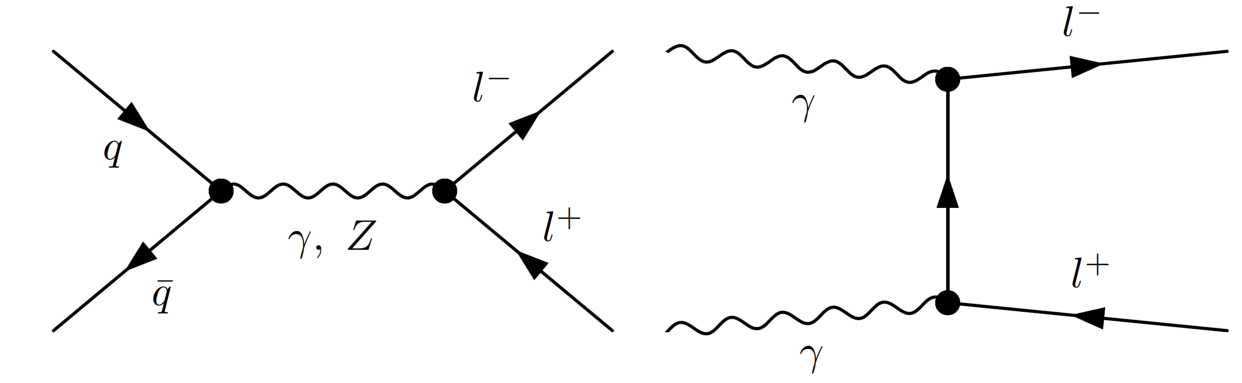
\includegraphics[width=8cm]{plots/photoninduced.pdf}
    \end{center}
  \caption{Two of the processes that contribute to lepton-pair
  production at hadron colliders at the Born level.}
\label{fig:photoninduced}
\end{figure}
%%%%%%%%%%%%%%%%%%%%%%%%%%%%%%%%%%%%%%%%%%%%%%%%%%%%%%%%%%%%%%%%

Deep-inelastic structure functions and PDF evolution will be performed
with the program {\tt APFEL}~\cite{Bertone:2013vaa}, which in its latest
version is accurate up to NNLO for the QCD corrections and up to
NLO for the QED corrections, as described in appendix~\ref{sec:appendixAPFEL}.
%
To be precise, this means that the DGLAP evolution equations are solved including
the splitting functions $P(\alpha_s,\alpha)$ up to $\mathcal{O}\lp \alpha_s^3\rp$ in the QCD
coupling and up to $\mathcal{O}\lp \alpha_s\alpha\rp$ in the QED coupling,
and that DIS coefficient functions include corrections up to $\mathcal{O}\lp \alpha_s^2\rp$
in QCD and up to $\mathcal{O}\lp \alpha^2\rp$ in QED.

Heavy quark (charm and bottom) mass effects in DIS structure functions are accounted
for using the FONLL-B(C) general-mass scheme~\cite{Forte:2010ta}
for the NLO (NNLO) fits.
%
As for the numerical values of the heavy quark masses in the pole scheme,
we take  $m_c=1.47~$GeV and $m_b=4.5~$GeV, consistent with the latest
PDG averages~\cite{Agashe:2014kda}.
%
With the same motivation, the strong (QED) coupling constant is chosen to be  $\alpha_s(m_Z)=0.118$
($\alpha(m_Z)=1/127$).
%
Let us recall that heavy quark structure functions with running masses
are also implemented in {\tt APFEL}~\cite{Bertone:2016ywq},
though their use should not lead to any difference for the determination of the photon PDF.
%
The charm PDF is generated perturbatively from light quarks and gluons using
the DGLAP equations.

For the calculation of high-mass Drell-Yan cross-sections,
we use the {\tt MadGraph5{\_}aMC@NLO}~\cite{Alwall:2014hca} program  v2.4.3,
which includes the contribution from photon initiated corrections,
and interfaced to {\tt APPLgrid}~\cite{Carli:2010rw} v1.4.70
and {\tt aMCfast}~\cite{Carli:2010rw} v1.3.00).
%
A tailored version of  {\tt APPLgrid} was used, allowing to account for
the contribution of photon-initiated processes.
%
The calculation is performed in the $n_f=5$ scheme neglecting the masses of the charm
and bottom quarks in the matrix elements, as appropriate for a high-scale processes
with $Q \gg m_Z$.

The ATLAS high-mass Drell-Yan 8 TeV measurements include both the one-dimensional
invariant mass distribution, $d\sigma/dm_{ll}$, as well as double-differential
distributions in $m_{ll}$ and $y_{ll}$, the rapidity of the dilepton pair,
$d^{2}\sigma/dm_{ll}d|y_{ll}|$, and in $m_{ll}$ and $\Delta\eta_{ll}$,
  the difference in 
  pseudorapidity between the lepton pair, $d^{2}\sigma/dm_{ll}\Delta\eta_{ll}$.
  %
  The {\tt MadGraph5{\_}aMC@NLO} theoretical predictions for these measurements
  follow the analysis cuts, including $m_{ll}\ge 116$ GeV,
  $\eta_l\le 2.5$, $p_T^l \ge 40(30)$ for the leading (sub-leading) lepton.

  
  For the invariant mass 
  distribution, there are 12 bins between 116 GeV and 1.5 TeV; and for both of the 
 the two-dimensional distributions, there are five different histograms, each one for a different invariant
 mass range: (a) 116 GeV < $m_{ll}$ < 150 GeV; (b) 150 GeV < $m_{ll}$ < 200 GeV; (c) 200 GeV < $m_{ll}$ < 300 GeV; (d) 300 GeV < $m_{ll}$ < 500 GeV; (e) 500 GeV < $m_{ll}$ < 1500 GeV.
 The {\tt APPLgrids} for the first three $m_{ll}$ intervals are divided into 12 bins with fixed bin 
width between $|y_{ll}^{mim}|$ ($|\Delta\eta_{ll}|$)  = 0.0 (0.0) and $|y_{ll}^{max}|$ ($|\Delta\eta_{ll}|$) = 2.4 (3.0), while the final two $m_{ll}$ intervals are divided into 6 bins with fixed bin width scanning the same $|y_{ll}|$ and $|\Delta\eta_{ll}|$ ranges.

Dynamical renormalization ($\mu_{R}$) and factorization ($\mu_{R}$) scales are used in the calculations 
and both are set to $m_{ll}$.
%
The theoretical calculations were validated by comparing both the NLO QCD + LO EW predictions and the 
LO PI predictions to those computed using the FEWZ 3.1 framework. These calculations are evaluated in the $G_{F}$ electroweak scheme, with the following values for the couplings:
 $\alpha_{S}$ = 0.118; $1/\alpha_{EW}$ = 1/127. The difference between the two predictions is at most 1${\%}$, for both the 1-dimensional and the 2-dimensional distributions.

In order to make a next-to-next-to-leading order (NNLO) fit k-factors ($k_{F}$) are computed matching
 the NLO QCD + LO EW cross sections to higher order (HO) calculations. These are computed using 
FEWZ, with the same input parameters as for the NLO computations. The $k_{F}$ are defined as:
\begin{equation}
  \label{eq:kfactor}
K \equiv\frac{\rm NNLO\  QCD  + NLO\  EW}{\rm NLO\  QCD + LO\  EW}
\end{equation}
In the calculation of the $K$-factor Eq.~(\ref{eq:kfactor}) the
MMHT2014 NNLO PDF set~\cite{Harland-Lang:2014zoa}
is used to compute both numerator and denominator, though
  results would change little if a different input PDF set was used.
  %
  These $K$-factors turn out to be close to 1, varying by at most 2\% in
  all the data bins.
  
